%Master File:lectures.tex
\newcommand{\rb}{\makebox(0,0){\textcolor{red}{$\bullet$}}}
\newcommand{\yb}{\makebox(0,0){\textcolor{yellow}{$\bullet$}}}
\newcommand{\wb}{\makebox(0,0){$\bullet$}}


\lesson{Singular Value Decomposition (SVD)}
\vspace{-1cm}
\begin{center}
\noindent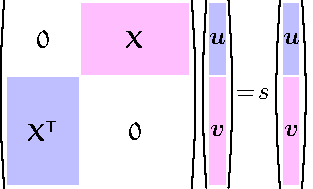
\includegraphics[height=90mm]{svd-1}
\end{center}
\keywords{Singular Valued Decomposition, SVD, general linear maps}
%%%%%%%%%%%%%%%%%%%%%%% Next Slide %%%%%%%%%%%%%%%%%%%%%%%
\renewcommand{\Outline}{%
\begin{slide}
\section[1]{Outline}

\begin{minipage}{12cm}\raggedright
  \begin{enumerate}\squeeze
    \outlineitem{Singular Value Decomposition}{svd}
    \outlineitem{General Linear Mappings}{glm}
    \outlineitem{Linear Regression Revisited}{lrr}
  \end{enumerate}
\end{minipage}\hfill
\begin{minipage}{10cm}
\ifnum\value{outlineitem}<3
  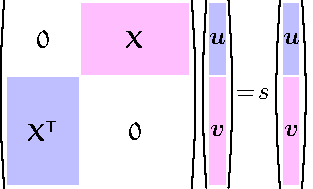
\includegraphics[width=10cm]{svd-1}
\fi
\ifnum\value{outlineitem}>2
  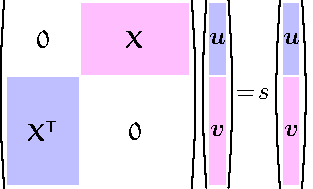
\includegraphics[width=10cm]{svd-1}
\fi
\end{minipage}
\end{slide}
\addtocounter{outlineitem}{1}
}

\setcounter{outlineitem}{1}

%%%%%%%%%%%%%%%%%%%%%%% Next Slide %%%%%%%%%%%%%%%%%%%%%%%
\Outline % SVD
\toptarget{firstoutline}
%%%%%%%%%%%%%%%%%%%%%%% Next Slide %%%%%%%%%%%%%%%%%%%%%%%

\begin{slide}
\section[-2]{Singular Valued Decomposition}

\pb
\begin{itemize}\squeeze
\item Consider an arbitrary $n\times m$ matrix $\mat{X}$, and construct
  the $(n+m)\times(n+m)$ symmetric matrix, $\mat{B}$, \pauseh\pauselevel{=1}
  \vspace*{-1cm}
  \begin{center}
    \multipdf[height=6cm]{svd}\pause
  \end{center}
  \vspace*{-1cm}
  $\binom{\bm{u}}{\bm{v}}$ is an eigenvector of $\mat{B}$ with eigenvalue $s$\pause
\item We observe that
  \begin{align*}
    \mat{X} \bm{v} &= s \bm{u} &
    \mat{X}^\tr \bm{u} &= s \bm{v} \pause\\
    \mat{X}^\tr \mat{X} \bm{v} &= s\,\mat{X}^\tr\bm{u} \pause = s^2 \bm{v}\pause &
    \mat{X} \mat{X}^\tr \bm{u} &= s\,\mat{X}\bm{v}\pause = s^2 \bm{u}\pause
  \end{align*}
\end{itemize}

\end{slide}

%%%%%%%%%%%%%%%%%%%%%%% Next Slide %%%%%%%%%%%%%%%%%%%%%%%

\begin{slide}
\section[-1]{Eigenvectors}

\begin{PauseHighLight}
  \begin{itemize}
  \item Note that as $\mat{X} \bm{v} = s \bm{u}$ and $\mat{X}^\tr
    \bm{u} = s \bm{v}$ then
    \begin{align*}
      \mat{X} (-\bm{v}) &= (-s) \bm{u}& 
      \mat{X}^\tr \bm{u} &= (-s) (-\bm{v})
    \end{align*}
    if $\binom{\bm{u}}{\bm{v}}$ is an eigenvector of $\mat{B}$ with
    eigenvalue $s$ then so is $\binom{\bm{u}}{-\bm{v}}$ 
    with eigenvalue $-s$\pause
  \item If $n<m$ then $\mat{X}^\tr\mat{X}$ is not full rank so some
    eigenvalues are zero\pause
  \item As a consequence $m-n$ vectors exist such that
    $\bm{X}\bm{v}=0$\pause
  \item The eigenvalues and eigenvectors are
    \begin{align*}
      n\times\left(s_i, \binom{\bm{u}_i}{\bm{v}_i}\right) \quad
      n\times\left(-s_i, \binom{\bm{u}_i}{-\bm{v}_i}\right) \quad
      m-n\times\left(0, \binom{0}{\bm{v}_k}\right) \pause
    \end{align*}
  \end{itemize}
\end{PauseHighLight}

\end{slide}

%%%%%%%%%%%%%%%%%%%%%%% Next Slide %%%%%%%%%%%%%%%%%%%%%%%

\begin{slide}
\section[-2]{Matrix Decomposition}

\begin{PauseHighLight}\squeeze
  \begin{itemize}
  \item Stacking the eigenvectors into a matrix
    \vspace*{-5mm}
    \begin{center}
      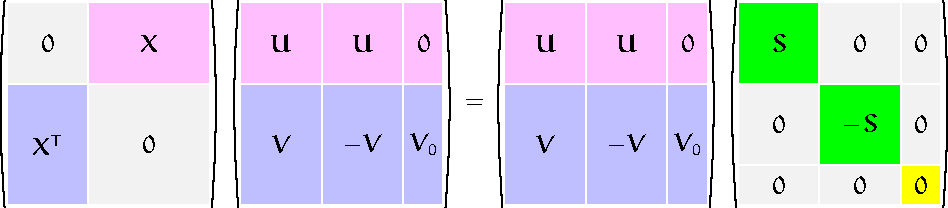
\includegraphics[height=4cm]{svdContinued-0}\pause
    \end{center}
    \vspace*{-5mm}
  \item Since the vectors $\binom{\bm{u}_i}{\bm{v}_i}$ are
    eigenvectors of a symmetric matrix they from an orthogonal matrix
    if they are normalised.\pause
  \item Multiply on the right by the transpose of the orthogonal matrix
    \vspace*{-5mm}
    \begin{center}
      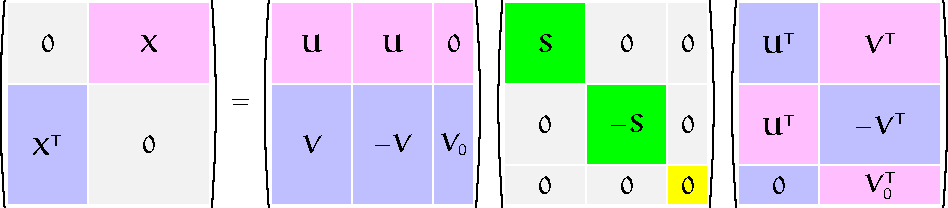
\includegraphics[height=4cm]{svdContinued-1}\pause
    \end{center}
  \end{itemize}
\end{PauseHighLight}


\end{slide}

%%%%%%%%%%%%%%%%%%%%%%% Next Slide %%%%%%%%%%%%%%%%%%%%%%%

\begin{slide}
  \section[-1.5]{Normalisation Subtlety}

  \begin{center}
    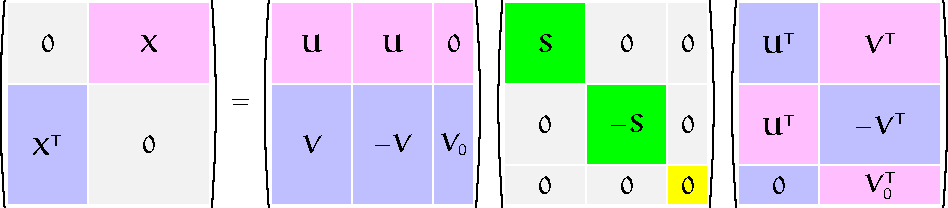
\includegraphics[height=4cm]{svdContinued-1}
  \end{center}
    \vspace*{-5mm}
  \begin{PauseHighLight}\squeeze
    \begin{itemize}
    \item Multiplying out we have
    \vspace*{-5mm}
    \begin{align*}
      \mat{X} &= 2\, \mat{U}\,\mat{S}\,\mat{V}^\tr &
      \mat{X}^\tr &=2\,  \mat{V}\,\mat{S}\,\mat{U}^\tr\pause
    \end{align*}
    \vspace*{-15mm}
    
  \item Now the vectors $\bm{u}_i$ and $\bm{v}_i$ form an orthogonal
    set as it  satisfy
    \vspace*{-5mm}
  \begin{align*}
    \mat{X}^\tr \mat{X} \bm{v} &= s^2 \bm{v} &
    \mat{X} \mat{X}^\tr \bm{u} &= s^2 \bm{u}\pause
  \end{align*}
  \vspace*{-15mm}
  
\item But they are not normalised (since $\binom{\bm{u}_i}{\bm{v}_i}$
  is normalised). If we define     $\tilde{\mat{U}} =
  \sqrt{2}\,\mat{U}$ and $\tilde{\mat{V}} = \sqrt{2}\,\mat{V}$
  we find
    \vspace*{-5mm}
  \begin{align*}
    \mat{X}   &=      \tilde{\mat{U}} \,\mat{S}\, \tilde{\mat{V}}^\tr &
    \mat{X}^\tr &= \tilde{\mat{V}} \,\mat{S}\, \tilde{\mat{U}}^\tr\pause
  \end{align*}
\end{itemize}
\end{PauseHighLight}

\end{slide}



%%%%%%%%%%%%%%%%%%%%%%% Next Slide %%%%%%%%%%%%%%%%%%%%%%%

\begin{slide}
\section{SVD}

\begin{PauseHighLight}
  \begin{itemize}
  \item Any matrix, $\mat{X}$, can be written as $\mat{X} =
    \mat{U}\,\mat{S}\,\mat{V}^\tr$
    \begin{itemize}
    \item $\mat{U}$, $\mat{V}$ are orthogonal matrices
    \item $\mat{S} = \mathrm{diag}(s_1, s_2,\ldots,s_n)$\pause
    \end{itemize}
  \item $s_i$ can always be chosen to be positive and are known as
    \emph{singular values}\pause
  \item Singular value decomposition applies to both square and
    non-square matrices---they describe general linear mappings\pause
  \end{itemize}
\end{PauseHighLight}

\end{slide}




%%%%%%%%%%%%%%%%%%%%%%% Next Slide %%%%%%%%%%%%%%%%%%%%%%%

\begin{slide}
\section{Finding SVD}

\begin{PauseHighLight}
  \begin{itemize}
  \item Most libraries will compute the SVD for you\pause
  \item They can do this by choosing the smaller of two matrices
    $\mat{X}\,\mat{X}^\tr$ and $\mat{X}^\tr\,\mat{X}$ and then compute
    the eigenvalues\pause
  \item The singular values are the square root of the eigenvalues
    (notice that $\mat{X}\,\mat{X}^\tr$ and $\mat{X}^\tr\,\mat{X}$ are
    both positive semi-definite so the eigenvalues will be
    non-negative)\pause
  \item It can compute the $\mat{U}$ matrix or $\bm{V}$ matrix by
    multiplying through by $\mat{X}$ or $\mat{X}^\tr$
    ($\mat{U} = \mat{X}\,\mat{V}\,\mat{S}^{-1}$ and $\mat{V} = \mat{X}^\tr
    \mat{U} \,\mat{S}^{-1}$)\pause 
  \item In practice to perform PCA most people subtract the mean from
    their data and then perform SVD\pause
  \end{itemize}
\end{PauseHighLight}

\end{slide}

%%%%%%%%%%%%%%%%%%%%%%% Next Slide %%%%%%%%%%%%%%%%%%%%%%%

\begin{slide}
\section[-2.5]{Economical Forms of SVD}

\begin{PauseHighLight}
  \begin{itemize}
  \item Often the rows or columns of the orthogonal matrices $\mat{U}$
    and $\mat{V}$ that are not associated with a singular value are
    ignored\pause
    \begin{center}
      \includegraphics[width=\linewidth]{twoForms1}\\
      \ \\
      \includegraphics[width=\linewidth]{twoForms2}
    \end{center}
  \item In Matlab these are obtained using
\begin{matlab}
  >> [U, S, V] = svd(X)
  >> [U, S, V] = svd(X,'econ'))
\end{matlab}\pause
  \end{itemize}
\end{PauseHighLight}

\end{slide}

%%%%%%%%%%%%%%%%%%%%%%% Next Slide %%%%%%%%%%%%%%%%%%%%%%%
\Outline % General Linear Mappings
%%%%%%%%%%%%%%%%%%%%%%% Next Slide %%%%%%%%%%%%%%%%%%%%%%%

\begin{slide}
\section{General Matrix}

\begin{PauseHighLight}
  \begin{itemize}
  \item Recall that we can compute the SVD for any matrix,
    $\mat{X}$\pause
  \item As matrices describe the most general linear mapping
    \begin{align*}
      \bm{v} \rightarrow \mathcal{T}[\bm{v}] = \mat{X}\bm{v}\pause
    \end{align*}
  \item We can use SVD to understand any linear mapping\pause
  \item Thus any linear mapping can be seen as a rotation followed by a
    squashing or expansion independently in each coordinate followed by
    another rotation\pause 
  \end{itemize}
\end{PauseHighLight}

\end{slide}

%%%%%%%%%%%%%%%%%%%%%%% Next Slide %%%%%%%%%%%%%%%%%%%%%%%

\begin{slide}
\section[-2]{Matrices}

\pb \pause
\begin{center}
  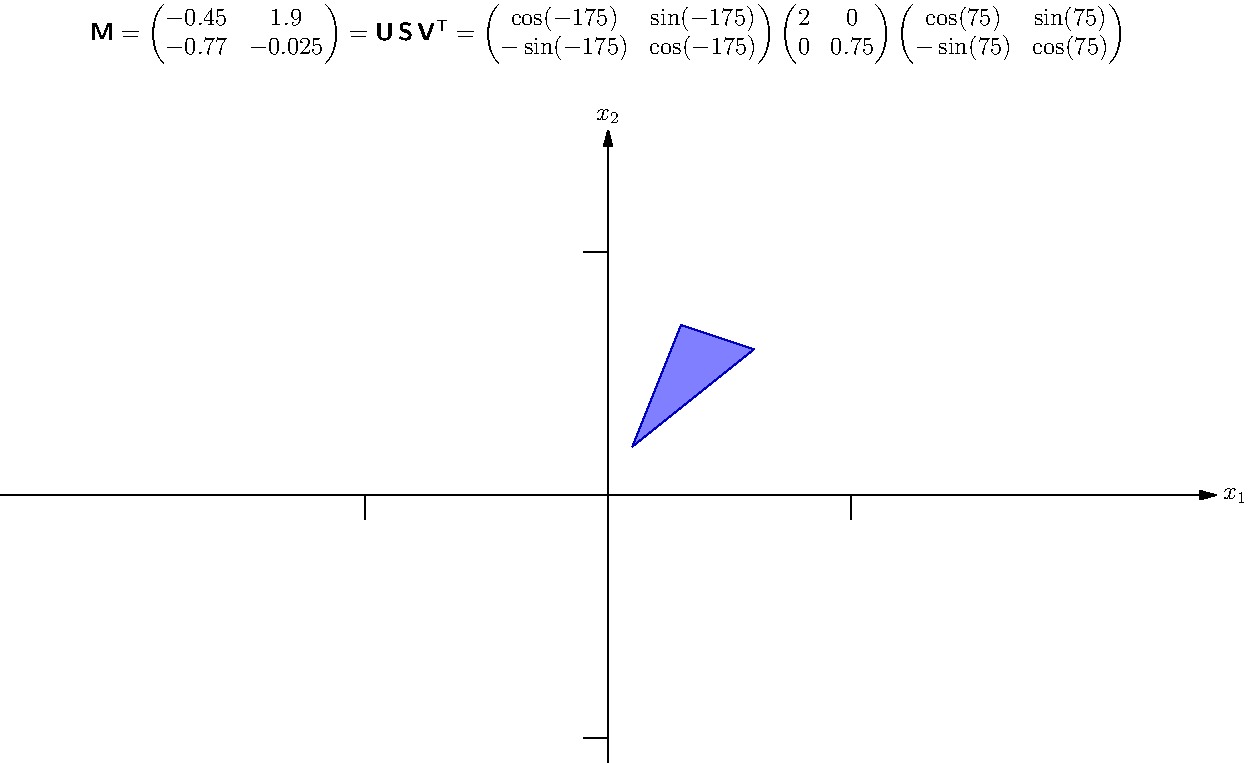
\includegraphics[width=\linewidth]{matrixPicture1}\mypl{1}
  \multido{\i=2+1}{4}{%
    \llap{\includegraphics[width=\linewidth]{matrixPicture\i}}\mypl{\i}}
\end{center}
\end{slide}



%%%%%%%%%%%%%%%%%%%%%%% Next Slide %%%%%%%%%%%%%%%%%%%%%%%

\begin{slide}
\section[-2]{Determinants}

\begin{PauseHighLight}
  \begin{itemize}
  \item The determinant, $|\mat{M}|$ of a matrix $\mat{M}$ is defined
    for square matrices\pause
  \item It describes the change in volume under the mapping\pause
  \item Now for any two matrices $|\mat{A}\,\mat{B}| =
    |\mat{A}|\,|\mat{B}|$\pause
  \item Thus
    \begin{align*}
      |\mat{M}| = |\mat{U}| \, |\mat{S}| \, |\mat{V}^\tr|\pause
    \end{align*}
  \item For and orthogonal matrix $|\mat{U}| = \pm 1$\pause
  \item Thus
    \begin{align*}
      |\mat{M}| = \pm |\mat{S}|\pause = \pm \prod_i s_i\pauseb
    \end{align*}
  \end{itemize}
\end{PauseHighLight}

\end{slide}


%%%%%%%%%%%%%%%%%%%%%%% Next Slide %%%%%%%%%%%%%%%%%%%%%%%

\begin{slide}
\section[-2]{Non-Square Matrices}

\begin{PauseHighLight}
  \begin{itemize}
  \item When the matrices are non-square then the matrix of singular
    value matrix will either
    \begin{itemize}
    \item Squash some directions to zero\pause
    \item Introduce new dimensions orthogonal to the vector
    \end{itemize}
  \end{itemize}
\end{PauseHighLight}
\begin{center}
  \includegraphics[width=\linewidth]{svdNonSquare}\pause
\end{center}
\begin{PauseHighLight}
  \begin{itemize}
  \item The rank of an arbitrary matrix is the number of non-zero singular values
    (also number of linearly independent rows or columns)\pause
  \end{itemize}
\end{PauseHighLight}

\end{slide}


%%%%%%%%%%%%%%%%%%%%%%% Next Slide %%%%%%%%%%%%%%%%%%%%%%%

\begin{slide}
\section[-2]{Duality Revisited}

\begin{PauseHighLight}
  \begin{itemize}
  \item If $\mat{X} = \mat{U}\,\mat{S}\,\mat{V}^\tr$ then
    \begin{align*}
      \mat{C} &= \mat{X}\, \mat{X}^\tr & \mat{D}  &= \mat{X}^\tr\, \mat{X}\pause\\
      &= \mat{U}\,\mat{S}\,\mat{V}^\tr\mat{V}\,\mat{S}^\tr\,\mat{U}^\tr &
      &=
        \mat{V}\,\mat{S}^\tr\,\mat{U}^\tr\mat{U}\,\mat{S}\,\mat{V}^\tr\pause\\
      &= \mat{U}\,(\mat{S}\mat{S}^\tr)\,\mat{U}^\tr  &
      &=
        \mat{V}\,(\mat{S}^\tr\,\mat{S})\,\mat{V}^\tr\pause                        
    \end{align*}
  \item If $\mat{X}$ is an $p\times m$ matrix then $\mat{S}\mat{S}^\tr$
    is a $p\times p$ diagonal matrix with elements $S_{ii}^2=s_i^2$\pause
  \item $\mat{S}^\tr\mat{S}$  is an $m\times m$ matrix  with elements
    $S_{ii}^2=s_i^2$\pause
  \item $\mat{U}$ and $\mat{V}$ are matrices of eigenvectors for
    $\mat{C}$ and $\mat{D}$\pause
  \item The eigenvalues are $\lambda_i = S_{ii}^2 = s_i^2$\pause
  \end{itemize}
\end{PauseHighLight}

\end{slide}

%%%%%%%%%%%%%%%%%%%%%%% Next Slide %%%%%%%%%%%%%%%%%%%%%%%

\begin{slide}
\section[-2]{$\mat{S}\mat{S}^\tr$ and $\mat{S}^\tr \mat{S}$}

\begin{PauseHighLight}\footnotesize
  \begin{align*}
    \mat{S} &=\begin{pmatrix}
        s_1 & 0 & \cdots & 0 & 0 & \cdots & 0 \\
        0 & s_2 &  \cdots & 0 & 0 & \cdots & 0 \\
        \vdots  & \vdots & \ddots & \vdots & \vdots & \ddots & \vdots \\
        0 & 0 & \cdots & s_m & 0 & 0 \cdots & 0
      \end{pmatrix}\pause
    \\
    \\
   \mat{S}^\tr \mat{S} &= \begin{pmatrix}
        s^2_1 & 0 &  \cdots & 0 & 0 & \cdots & 0 \\
        0 & s^2_2 &  \cdots & 0 & 0 & \cdots & 0 \\
        \vdots & \vdots  & \ddots & \vdots & \vdots & \ddots & \vdots \\
        0 & 0 & \cdots & s^2_m & 0 & 0 \cdots & 0 \\
        0 & 0 & \cdots & 0 & 0 & 0 \cdots & 0\\
        \vdots & \vdots & \cdots & \vdots & \vdots & \vdots \cdots & \vdots\\
        0 & 0 & \cdots & 0 & 0 & 0 \cdots & 0
      \end{pmatrix}\pause
    \\
    \\
    \mat{S}\,\mat{S}^\tr &= \begin{pmatrix}
        s^2_1 & 0 & \cdots & 0  \\
        0 & s^2_2 &  \cdots & 0 \\
        \vdots  & \vdots & \ddots & \vdots  \\
        0 & 0 & \cdots & s^2_m
      \end{pmatrix}\pause
  \end{align*}
\end{PauseHighLight}


\end{slide}


%%%%%%%%%%%%%%%%%%%%%%% Next Slide %%%%%%%%%%%%%%%%%%%%%%%

\begin{slide}
\section{Having A Go}

\begin{PauseHighLight}
  \begin{itemize}
  \item It's really easy to verify this in MATLAB or OCTAVE\pause
\begin{matlab}
>> X = rand(3,2)
>> [U, S, V] = svd(X)
>> U*S*V'
>> U(:,1)'*U(:,2)
>> U'*U
>> U*U'
>> [Ua,L] = eig(X*X')
>> S*S'
\end{matlab}\pause
  \item Test yourself!\pause
  \end{itemize}
\end{PauseHighLight}

\end{slide}


%%%%%%%%%%%%%%%%%%%%%%% Next Slide %%%%%%%%%%%%%%%%%%%%%%%
\Outline % Linear Regression Revisited
%%%%%%%%%%%%%%%%%%%%%%% Next Slide %%%%%%%%%%%%%%%%%%%%%%%

\begin{slide}
\section{Linear Regression}

\begin{PauseHighLight}
  \begin{itemize}
  \item Given a set of data $\mathcal{D}= \{(\bm{x}_i, y_i)|k=1,\,2,\,\ldots,\, m\}$\pause
  \item In linear regression we try to fit a linear model
    \begin{align*}
      f(\bm{x}| \bm{w}) = \bm{x}^\tr \bm{w}\pause
    \end{align*}
  \item Which we fit by minimising the squared error loss
    \begin{align*}
      L(\bm{w}) = \sum_{k=1}^m \left(f(\bm{x}_i| \bm{w}) - y_i\right)^2\pause
    \end{align*}
  \end{itemize}
\end{PauseHighLight}

\end{slide}

%%%%%%%%%%%%%%%%%%%%%%% Next Slide %%%%%%%%%%%%%%%%%%%%%%%

\begin{slide}
\section{Matrix Form}

\begin{PauseHighLight}
  \begin{itemize}
    \item In matrix from we write $L(\bm{w})= \left\| \mat{X}\,\bm{w} -
      \bm{y} \right\|^2$
    \begin{align*}
      \mat{X} &=
                \begin{pmatrix}
                  \bm{x}_1^\tr \\ \bm{x}_2^\tr \\ \vdots \\ \bm{x}_m^\tr
                \end{pmatrix}
              &
      \bm{y} &=
               \begin{pmatrix}
                 y_1 \\ y_2, \\ \vdots \\ y_m
               \end{pmatrix}\pause
    \end{align*}
  \item Then $\grad L(\bm{w}^*)=0$ implies
    \begin{align*}
      \bm{w}^* = \left(\mat{X}^\tr\,\mat{X}\right)^{-1} \mat{X}^\tr \bm{y}\pause
      = \mat{X}^{+} \bm{y}
    \end{align*}
  \item This is known as the pseudo-inverse\pause
  \end{itemize}
\end{PauseHighLight}

\end{slide}

%%%%%%%%%%%%%%%%%%%%%%% Next Slide %%%%%%%%%%%%%%%%%%%%%%%

\begin{slide}
\section[-2]{Using SVD}

\begin{PauseHighLight}
  \begin{itemize}
  \item Using $\mat{X} = \mat{U}\,\mat{S}\,\mat{V}^\tr$ then
    \begin{align*}
      \mat{X}^{+} &= \left(\mat{X}^\tr\,\mat{X}\right)^{-1} \mat{X}^\tr \pause\\
      &=  \left(\mat{V}\,\mat{S}^\tr\mat{S} \mat{V}^\tr\right)^{-1}
        \mat{V}\,\mat{S}^\tr\,\mat{U}^\tr\pause \\
      &= \mat{V}\,\left(\mat{S}^\tr\mat{S}\right)^{-1}
        \mat{V}^\tr\,\mat{V}\,\mat{S}^\tr\,\mat{U}^\tr\pause\\
      &= \mat{V}\,\left(\mat{S}^\tr\mat{S}\right)^{-1}\mat{S}^\tr\,\mat{U}^\tr\pause
      = \mat{V}\,\mat{S}^{+} \mat{U}^\tr\pause
    \end{align*}
  \item If $m>p${\small
    \begin{align*}
      \mat{X}^\tr &= \begin{pmatrix}
        \textcolor{gray}{\rule{8pt}{4cm}} &
        \textcolor{gray}{\rule{8pt}{4cm}} &
        \textcolor{gray}{\rule{8pt}{4cm}} &
        \textcolor{gray}{\rule{8pt}{4cm}} &
        \textcolor{gray}{\rule{8pt}{4cm}} &
        \textcolor{gray}{\rule{8pt}{4cm}} &
        \textcolor{gray}{\rule{8pt}{4cm}} &
        \textcolor{gray}{\rule{8pt}{4cm}} 
      \end{pmatrix},\pause
      \mat{S}^\tr &= \begin{pmatrix}
        s_1 & 0 & 0 & \cdots & 0 & 0 & \cdots & 0 \\
        0 & s_2 & 0 & \cdots & 0 & 0 & \cdots & 0 \\
        0 & 0 & s_3 & \cdots & 0 & & 0 \cdots & 0 \\
        \vdots & \vdots & \vdots & \ddots & \vdots & \vdots & \ddots & \vdots \\
        0 & 0 & 0 & \cdots & s_p & 0 & 0 \cdots & 0
        \end{pmatrix}\pause
    \end{align*}}
  \end{itemize}
\end{PauseHighLight}

\end{slide}


%%%%%%%%%%%%%%%%%%%%%%% Next Slide %%%%%%%%%%%%%%%%%%%%%%%

\begin{slide}
\section{Pseudo-Inverse of $\mat{S}$}

\begin{PauseHighLight}
\begin{align*}
  \mat{S}^\tr\mat{S} &= \begin{pmatrix}
        s_1^{2} & 0 & \cdots & 0  \\
        0 & s_2^{2} & \cdots & 0  \\
        \vdots & \vdots & \ddots & \vdots\\
        0 & 0 & \cdots & s_p^{2}
        \end{pmatrix}\pause &
  \left(\mat{S}^\tr\mat{S}\right)^{-1}&= \begin{pmatrix}
        s_1^{-2} & 0 & \cdots & 0  \\
        0 & s_2^{-2} & \cdots & 0  \\
        \vdots & \vdots & \ddots & \vdots\\
        0 & 0 & \cdots & s_p^{-2}
        \end{pmatrix}\pause
\end{align*}
\begin{align*}
  \mat{S}^{+}  = \left(\mat{S}^\tr\mat{S}\right)^{-1}\mat{S}^\tr\pause
  = \begin{pmatrix}
        s_1^{-1} & 0 & 0 & \cdots & 0 & 0 & \cdots & 0 \\
        0 & s_2^{-1} & 0 & \cdots & 0 & 0 & \cdots & 0 \\
        0 & 0 & s_3^{-1} & \cdots & 0 & & 0 \cdots & 0 \\
        \vdots & \vdots & \vdots & \ddots & \vdots & \vdots & \ddots & \vdots \\
        0 & 0 & 0 & \cdots & s_p^{-1} & 0 & 0 \cdots & 0
        \end{pmatrix}\pause
\end{align*}
\end{PauseHighLight}
\end{slide}

%%%%%%%%%%%%%%%%%%%%%%% Next Slide %%%%%%%%%%%%%%%%%%%%%%%

\begin{slide}
\section{Ill-Conditioned Data Matrix}

\begin{PauseHighLight}
  \begin{itemize}
  \item Recall that
    \begin{align*}
      \bm{w}^* = \mat{X}^{+} \bm{y} =  \mat{V}\,\mat{S}^{+} \mat{U}^\tr \bm{y}\pause
    \end{align*}
  \item If any of the singular values of $\mat{X}$ are small then
    $\mat{S}^{+}$ will magnify components in that direction\pause
  \item Any errors in the target $\bm{y}$ will be magnified\pause
  \item This leads to poor weights\pause
  \end{itemize}
\end{PauseHighLight}

\end{slide}

%%%%%%%%%%%%%%%%%%%%%%% Next Slide %%%%%%%%%%%%%%%%%%%%%%%

\begin{slide}
\section{Regularisation}

\begin{PauseHighLight}
  \begin{itemize}
  \item Consider linear regression with a regulariser
    \begin{align*}
      \mathcal{L}(\bm{w})
      &=  \left\| \mat{X}\,\bm{w} - \bm{y} \right\|^2 + \eta \, \|\bm{w}\|^2
      \\
      &= \bm{w}^\tr \left(\mat{X}^\tr \mat{X} + \eta \, \mat{I}
        \right) \bm{w}  - 2 \, \bm{w}^\tr \, \mat{X}^\tr \, \bm{y} +
        \bm{y}^\tr\,\bm{y} \pause
    \end{align*}
  \item Thus
    \begin{align*}
      \grad \mathcal{L}(\bm{w}) = 2 \,
      \left(\mat{X}^\tr \mat{X} + \eta \, \mat{I} \right) \bm{w}
      - 2 \, \mat{X}^\tr \, \bm{y}\pause
    \end{align*}
  \item and $\grad \mathcal{L}(\bm{w}^*)=0$ gives
    \begin{align*}
      \bm{w}^* = \left(\mat{X}^\tr \mat{X} + \eta \, \mat{I}
      \right)^{-1} \mat{X}^\tr \, \bm{y}\pause
    \end{align*}
  \end{itemize}
\end{PauseHighLight}

\end{slide}

%%%%%%%%%%%%%%%%%%%%%%% Next Slide %%%%%%%%%%%%%%%%%%%%%%%

\begin{slide}
  \section[-1]{Regularisation Continued}

\begin{PauseHighLight}
  \begin{itemize}
  \item Using $\mat{X} = \mat{U}\,\mat{S}\,\mat{V}^\tr$
    \begin{align*}
      \bm{w}^*
      &= \left(\mat{X}^\tr \mat{X} + \eta \, \mat{I}
        \right)^{-1} \mat{X}^\tr \, \bm{y}\pause \\
      &= \mat{V} \left( \mat{S}^\tr\mat{S} +  \eta \, \mat{I} \right)^{-1}
        \mat{S}^\tr \mat{U}^\tr \bm{y}\pause
    \end{align*}
  \item where
    \begin{align*}
      \left( \mat{S}^\tr\mat{S} + \eta \,  \mat{I} \right)^{-1}
      \mat{S}^\tr =
      \begin{pmatrix}
        \frac{s_1}{s_1^2 + \eta} & 0 & 0 & \cdots & 0 & 0 & \cdots & 0 \\
          0 & \frac{s_2}{s_2^2 + \eta} & 0 & \cdots & 0 & 0 & \cdots & 0 \\
          0 & 0 & \frac{s_3}{s_3^2 + \eta} & \cdots & 0 & & 0 \cdots & 0 \\
        \vdots & \vdots & \vdots & \ddots & \vdots & \vdots & \ddots & \vdots \\
          0 & 0 & 0 & \cdots & \frac{s_p}{s_p^2 + \eta} & 0 & 0 \cdots & 0
       \end{pmatrix}\pause
    \end{align*}
  \end{itemize}
\end{PauseHighLight}

\end{slide}

%%%%%%%%%%%%%%%%%%%%%%% Next Slide %%%%%%%%%%%%%%%%%%%%%%%

\begin{slide}
\section[-2]{Effect of Regularisation}

\begin{PauseHighLight}
  \begin{itemize}
  \item Without regularisation if $s_i=0$ the problem would be ill-posed (even $\mat{S}^+$
    does not exist since $s_i^{-1}$ would be ill defined) and if $s_i$
    is small then $\mat{S}^+$ is ill conditioned\pause
  \item Using $\hat{\mat{S}}^+
    =(\mat{S}^\tr\mat{S}+\eta)^{-1}\,\mat{S}^\tr$ instead of
    $\mat{S}^+$ then 
    \begin{center}
     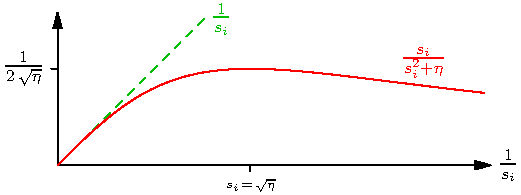
\includegraphics[width=0.8\textwidth]{linregressreg} \pause
   \end{center}
   \vspace*{-2ex}
  \item Regularisation makes the machine much more stable (reduces the
    variance)\pause
  \end{itemize}
\end{PauseHighLight}

\end{slide}



%%%%%%%%%%%%%%%%%%%%%%% Next Slide %%%%%%%%%%%%%%%%%%%%%%%

\begin{slide}
\section[-2]{Summary}

\begin{PauseHighLight}
  \label{last}

  \begin{itemize}
  \item Any matrix can be decomposed as
    $\mat{X}=\mat{U}\mat{S}\mat{V}^\tr$ where
    \begin{itemize}
    \item $\mat{U}$ and $\mat{V}$ are orthogonal (rotation matrices)\pause
    \item $\mat{S}=\diag(s_1, \ldots, s_n)$ is a diagonal
      matrix of positive singular values\pause
    \end{itemize}
  \item This describes the most general linear transform\pause
  \item The transform exploits the duality between $\mat{X}\,\mat{X}^\tr$
    and $\mat{X}^\tr\,\mat{X}$\pause
  \item In linear regression the pseudo-inverse involves the reciprocal of
    the singular values, which can lead to poor generalisation\pause
  \item Regularisation improves the conditioning of the ``inverse'' matrix\pause
  \end{itemize}
\end{PauseHighLight}
\end{slide}



%%% Local Variables:
%%% TeX-master: "lectures"
%%% End:
